\documentclass[12pt]{article}
\input{/Users/circle/Documents/博一下/homework/setting.tex}
\setcounter{secnumdepth}{2}
\usepackage{autobreak}
\usepackage{amsmath}
\setlength{\parindent}{2em}
\graphicspath{{../}}
\ziju{0.1pt}


%pdf文件设置
\hypersetup{
	pdfauthor={袁磊祺},
	pdftitle={计算流体力学作业3}
}

\title{
		\vspace{-1in} 	
		\usefont{OT1}{bch}{b}{n}
		\normalfont \normalsize \textsc{\LARGE Peking University}\\[0.2cm] % Name of your university/college \\ [25pt]
		\horrule{0.5pt} \\[0.2cm]
		\huge \bfseries{计算流体力学作业3} \\[-0.2cm]
		\horrule{2pt} \\[0.2cm]
}
\author{
		\normalfont 								\normalsize
		College of Engineering \quad 2001111690  \quad 袁磊祺\\	\normalsize
        \today
}
\date{}

\begin{document}

\input{setc.tex}

\maketitle

\section{Cauchy问题的解}

利用特征线理论分析问题
\begin{equation}
	\begin{cases}
		u_{t}+a(u) u_{x}=0, & x \in \mathbb{R},\ t>0, \\
		u(x, 0)=u_{0}(x), & x \in \mathbb{R}.
	\end{cases}
	\label{eq:10}
\end{equation}
并给出(光滑的)解.

{\bfseries 解:}
$u_{t}+a(u) u_{x}=0, u(x, 0)=u_{0}(x) .$ 问题转化为
\begin{equation}
	\begin{cases}
		\frac{\dif x}{\dif t}=a(u), \\
		x(0)=x_{0}.
	\end{cases}
	\quad
	\begin{cases}
		\frac{\dif u}{\dif t}=0, \\
		u(0)=u_{0}\left(x_{0}\right).		
	\end{cases}
\end{equation}

由上述ODE初值问题得
\begin{equation}
	u(x,t) = u_0(x_0),
	\label{eq:11}
\end{equation}
\begin{equation}
	x=x_{0}+a(u_0(x_0))t=x_{0}+a(u(x,t))t,
	\label{eq:111}
\end{equation}
$x_0$依赖于给定的点$(x,t)$,
\begin{equation}
	u(x, t)=u_{0}\left(x-a(u_0(x_0))t\right)=u_{0}\left(x-a(u_0(x_0(x,t)))t\right)=u_{0}\left(x-a(u(x,t))t\right).
	\label{eq:12}
\end{equation}

由\cref{eq:10}得
\begin{equation}
	u_{t}=u_{0}^{\prime}\left(x_{0}\right) \frac{\partial x_{0}}{\partial t}, \quad u_{x}=u_{0}^{\prime}\left(x_{0}\right) \frac{\partial x_{0}}{\partial x}
	\label{eq:121}
\end{equation}

将\cref{eq:111} 的第一等号两端分别对$t$和 $x$ 求导, 得

\begin{gather}
a\left(u_{0}\left(x_{0}\right)\right)+\left[1+a^{\prime} \cdot u_{0}^{\prime}\left(x_{0}\right) \cdot t\right] \frac{\partial x_{0}}{\partial t}=0 
\label{eq:130}
\\
\left(1+a^{\prime} u_{0}^{\prime}\left(x_{0}\right) t\right) \frac{\partial x_{0}}{\partial x}=1
\label{eq:13}
\end{gather}

从\cref{eq:130,eq:13}得
\begin{equation}
	\frac{\partial x_{0}}{\partial t}=-\frac{a\left(u_{0}\left(x_{0}\right)\right)}{1+\left(a^{\prime} u_{0}^{\prime}\right)_{x_{0}} t}, \quad \frac{\partial x_{0}}{\partial x}=\frac{1}{1+\left(a^{\prime} u_{0}^{\prime}\right)_{x_{0}} t}.
\end{equation}

将其代入\cref{eq:121}知
\begin{equation}
	u_{t}+a(u) u_{x}=0.
\end{equation}

$t=0$时
\begin{equation}
	u(0)=u_{0}\left(x_{0}\right),
\end{equation}
所以\cref{eq:12}满足\cref{eq:10}.

\section{无黏 Burgers 方程的定解问题}

\begin{equation}
	\begin{cases}
		u_t+(0.5 u^2)_x=0, \\
		u_0(x) = \cos(\pi x),\quad x \in [-1,1].
	\end{cases}
\end{equation}


此时$a(u)=u$,爆破点
\begin{equation}
	t^* = - \frac{1}{a'u_0'} = \frac{1}{\pi \sin(\pi x_0)},
\end{equation}
只在$x>0$的部分会出现爆破,最快达到爆破的点为$x_0=0.5$,经历时间$t_0^*=\frac{1}{\pi}$.

初始图像如\cref{fig:0}所示,当其运动到爆破的时候如\cref{fig:1} 所示,可以发现右边的线已经和$x$轴垂直了。

\begin{figure}[htp]
	\centering
	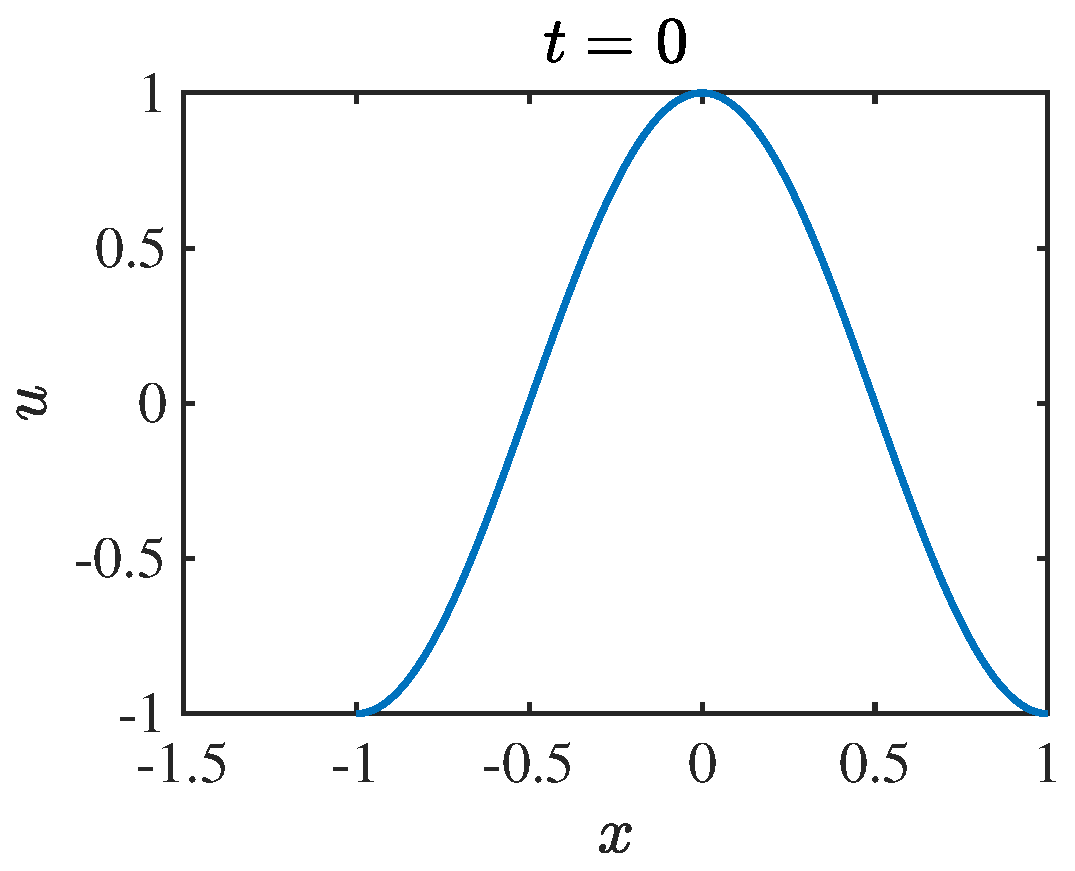
\includegraphics[width=7cm]{0.eps}
	\caption{$t=0$。}
	\label{fig:0}
\end{figure}

\begin{figure}[htp]
	\centering
	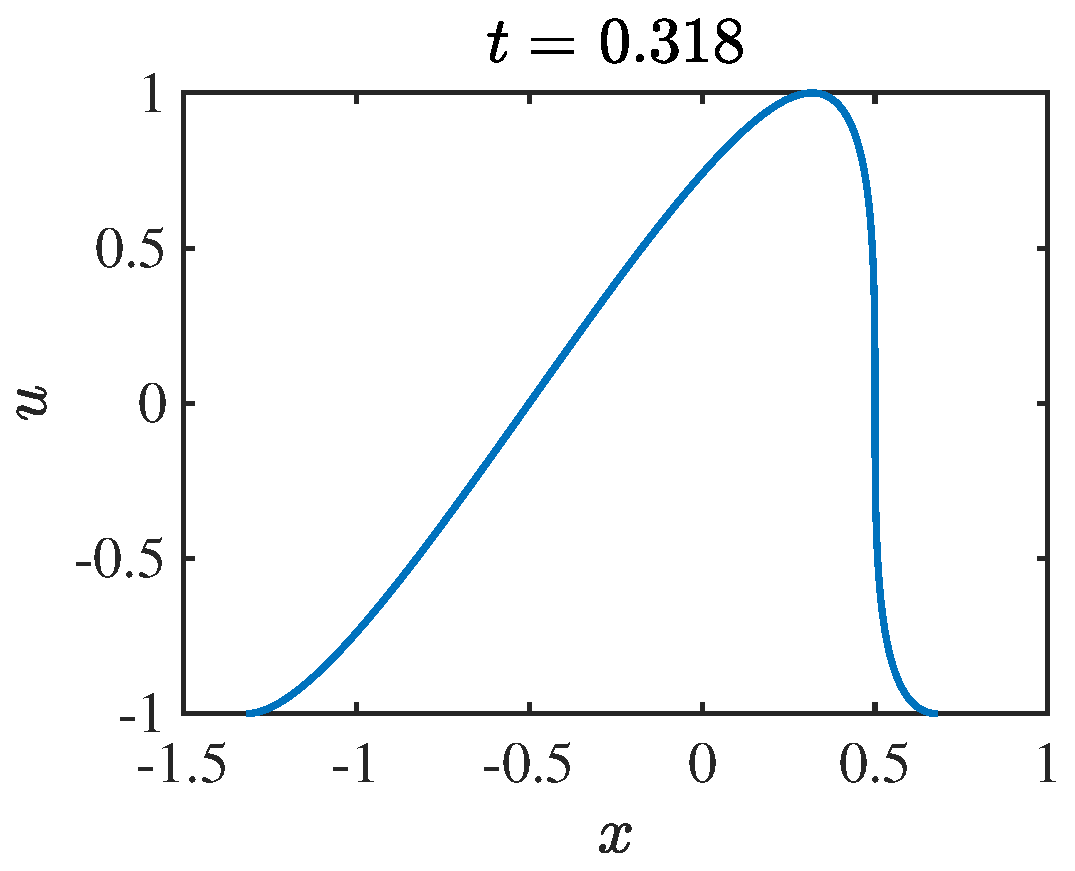
\includegraphics[width=7cm]{1.eps}
	\caption{$t=\frac{1}{\pi}$。爆破时刻。}
	\label{fig:1}
\end{figure}

\section{Burgers 方程 Riemann 问题的弱解}

弱解满足的方程为
\begin{equation}
	\int_{0}^{+\infty} \int_{-\infty}^{+\infty}\left[\phi_{t} \boldsymbol{U}+\phi_{x} \boldsymbol{F}(\boldsymbol{U})\right] \dif x \dif t=-\int_{-\infty}^{+\infty} \phi(x, 0) \boldsymbol{U}(x, 0) \dif x.
\end{equation}

对Burgers 方程有
\begin{equation}
	\int_{0}^{+\infty} \int_{-\infty}^{+\infty}\left[\phi_{t} {u}+\phi_{x} \frac{1}{2}u^2\right] \dif x \dif t=-\int_{-\infty}^{+\infty} \phi(x, 0) {u}(x, 0) \dif x.
\end{equation}

\subsection{激波弱解}


\begin{equation}
	u(x, t)=
	\begin{cases}
		u_{L}, & x<s t, \\
		u_{R}, & x>s t	.
	\end{cases}
\end{equation}
其中
\begin{equation}
	s=\frac{u_L+u_R}{2}.
\end{equation}

\begin{align}
	& \int_{0}^{+\infty} \int_{-\infty}^{+\infty}\left[\phi_{t} {u}+\phi_{x} \frac{1}{2}u^2\right] \dif x \dif t \\
	= & \int_{0}^{+\infty} \int_{-\infty}^{+\infty}\phi_{t} {u} \dif x \dif t + \int_{0}^{+\infty} \int_{-\infty}^{+\infty}\phi_{x} \frac{1}{2}u^2 \dif x \dif t \\
	= & -\int_{-\infty}^{+\infty} \phi(x, 0) {u}(x, 0) \dif x +  \int_{0}^{+\infty} \phi(x, x/s) \left(u_L-u_R\right) \dif x\\
	& + \frac{1}{2} \int_{0}^{+\infty} \phi(st, t) \left(u_L^2-u_R^2\right) \dif t\\
	= & -\int_{-\infty}^{+\infty} \phi(x, 0) {u}(x, 0) \dif x +  s \int_{0}^{+\infty} \phi(x, x/s) \left(u_L-u_R\right) \dif\, (x/s)\\
	& + \frac{1}{2} \int_{0}^{+\infty} \phi(st, t) \left(u_L^2-u_R^2\right) \dif t\\
	= & -\int_{-\infty}^{+\infty} \phi(x, 0) {u}(x, 0) \dif x.
\end{align}

\subsection{$u_L<u_R$弱解}


\begin{equation}
	u(x, t)=
	\begin{cases}
		u_{L}, & x<s t, \\
		u_{R}, & x>s t	.
	\end{cases}
\end{equation}
其中
\begin{equation}
	s=\frac{u_L+u_R}{2}.
\end{equation}

同样的
\begin{align}
	& \int_{0}^{+\infty} \int_{-\infty}^{+\infty}\left[\phi_{t} {u}+\phi_{x} \frac{1}{2}u^2\right] \dif x \dif t \\
	= & \int_{0}^{+\infty} \int_{-\infty}^{+\infty}\phi_{t} {u} \dif x \dif t + \int_{0}^{+\infty} \int_{-\infty}^{+\infty}\phi_{x} \frac{1}{2}u^2 \dif x \dif t \\
	= & -\int_{-\infty}^{+\infty} \phi(x, 0) {u}(x, 0) \dif x +  \int_{0}^{+\infty} \phi(x, x/s) \left(u_L-u_R\right) \dif x\\
	& + \frac{1}{2} \int_{0}^{+\infty} \phi(st, t) \left(u_L^2-u_R^2\right) \dif t\\
	= & -\int_{-\infty}^{+\infty} \phi(x, 0) {u}(x, 0) \dif x +  s \int_{0}^{+\infty} \phi(x, x/s) \left(u_L-u_R\right) \dif\, (x/s)\\
	& + \frac{1}{2} \int_{0}^{+\infty} \phi(st, t) \left(u_L^2-u_R^2\right) \dif t\\
	= & -\int_{-\infty}^{+\infty} \phi(x, 0) {u}(x, 0) \dif x.
\end{align}

\subsection{稀疏波弱解}

\begin{equation}
	u(x, t)=
	\begin{cases}
		u_{L}, & x<s_{m} t \\
		u_{m}, & s_{m} t \leq x \leq u_{m} t \\
		\frac{x}{t}, & u_{m} t \leq x \leq u_{R} t \\
		u_{R}, & x>u_{R} t
	\end{cases}
\end{equation}
也是一个弱解, 其中 $u_{m} \in\left[u_{L}, u_{R}\right]$ 为任意, $s_{m}=\frac{u_{L}+u_{m}}{2} .$ 不妨设$u_L>0,\ u_R>0$.
\begin{align}
	& \int_{0}^{+\infty} \int_{-\infty}^{+\infty}\left[\phi_{t} {u}+\phi_{x} \frac{1}{2}u^2\right] \dif x \dif t \\
	= & -\int_{-\infty}^{+\infty} \phi(x, 0) {u}(x, 0) \dif x + \int_{0}^{+\infty} \left( - u_{L} \phi\left(x, \frac{x}{s_{m}}\right)+u_{m} \phi\left(x, \frac{x}{s_{m}}\right)\right. \\
	&\left.-u_{m} \phi\left(x, \frac{x}{u_{m}}\right)+\int_{\frac{x}{u_{R}}}^{\frac{x}{u_m}} \phi_{t} \frac{x}{t} \dif t + u_{R} \phi\left(x, \frac{x}{u_{R}}\right) \right) \dif x\\
	& + \int_{0}^{+\infty} \frac{1}{2} \left(- u_{R}^{2} \phi\left(u_{R} t, t\right)+\int_{u_{m} t}^{u_{R} t}  \frac{x^{2}}{t^{2}} \phi_{x}(x, t) \dif x +  u_{m}^{2} \phi\left(u_{m} t, t\right) + \left(u_{L}^{2}- u_{m}^{2}\right)  \phi\left(s_{m} t, t\right) \right) \dif t.\\
	= & -\int_{-\infty}^{+\infty} \phi(x, 0) {u}(x, 0) \dif x + \int_{0}^{+\infty} \left(-u_{m} \phi\left(x, \frac{x}{u_{m}}\right)+\int_{\frac{x}{u_{R}}}^{\frac{x}{u_m}} \phi_{t} \frac{x}{t} \dif t + u_{R} \phi\left(x, \frac{x}{u_{R}}\right) \right) \dif x\\
	& + \int_{0}^{+\infty} \frac{1}{2} \left(- u_{R}^{2} \phi\left(u_{R} t, t\right)+\int_{u_{m} t}^{u_{R} t}  \frac{x^{2}}{t^{2}} \phi_{x} \dif x +  u_{m}^{2} \phi\left(u_{m} t, t\right)  \right) \dif t.
\end{align}
其中
\begin{align}
	\int_{\frac{x}{u_{R}}}^{\frac{x}{u_m}} \phi_{t} \frac{x}{t} \dif t = & 	\left.\left(\frac{x}{t} \phi\right)\right|_{t=\frac{x}{u_{R}}} ^{t=\frac{x}{u_{m}}}+\int_{\frac{x}{u_{R}}}^{\frac{x}{u_{m}}} \frac{x}{t^{2}} \phi \dif t \\
	= & u_m \phi(x,\frac{x}{u_m}) -  u_R \phi(x,\frac{x}{u_R})+\int_{\frac{x}{u_{R}}}^{\frac{x}{u_{m}}} \frac{x}{t^{2}} \phi \dif t,
\end{align}
\begin{align}
	\int_{u_{m} t}^{u_{R} t}  \frac{x^{2}}{t^{2}} \phi_{x} \dif x = & 	\left.\frac{x^{2}}{t^{2}} \phi\right|_{x=u_{m} t} ^{x=u_{R} t}-\int_{u_{m} t}^{u_{R} t} \frac{2 x}{t^{2}} \phi \dif x\\
	= & u_R^2 \phi(u_Rt,t) -  u_m^2 \phi(u_mt,t)-\int_{u_{m} t}^{u_{R} t} \frac{2 x}{t^{2}} \phi \dif x.
\end{align}
所以
\begin{align}
	& \int_{0}^{+\infty} \int_{-\infty}^{+\infty}\left[\phi_{t} {u}+\phi_{x} \frac{1}{2}u^2\right] \dif x \dif t \\
	= & -\int_{-\infty}^{+\infty} \phi(x, 0) {u}(x, 0) \dif x + \int_{0}^{+\infty} \int_{\frac{x}{u_{R}}}^{\frac{x}{u_{m}}} \frac{x}{t^{2}} \phi \dif t  \dif x - \int_{0}^{+\infty}  \int_{u_{m} t}^{u_{R} t} \frac{x}{t^{2}} \phi \dif x \dif t\\
	= & -\int_{-\infty}^{+\infty} \phi(x, 0) {u}(x, 0) \dif x.
\end{align}\qed

\section{线化气体动力学方程}

线化气体动力学方程组
\begin{equation}
	\begin{cases}
		\frac{\partial \rho}{\partial t}+\rho_{0} \frac{\partial u}{\partial x}=0, \\
		\frac{\partial u}{\partial t}+\frac{a_{0}^{2}}{\rho_{0}} \frac{\partial \rho}{\partial x}=0.
	\end{cases}
\end{equation}



\subsection{一般初值问题的解}

\begin{equation}
	\boldsymbol{U}_{t}+\boldsymbol{A} \boldsymbol{U}_{x}=0, \quad \boldsymbol{U}=\left(\begin{array}{l}
		\rho \\
		u
		\end{array}\right), \quad \boldsymbol{A}=\left(\begin{array}{cc}
		0 & \rho_{0} \\
		a_{0}^{2} / \rho_{0} & 0
		\end{array}\right)
\end{equation}
其中
\begin{equation}
	\boldsymbol{R}^{(1)}=\left(\begin{array}{c}
		\rho_{0} \\
		-a_{0}
		\end{array}\right), \quad \boldsymbol{R}^{(2)}=\left(\begin{array}{c}
		\rho_{0} \\
		a_{0}
		\end{array}\right), \begin{array}{l}
		\lambda_{1}=-a_{0} \\
		\lambda_{2}=a_{0}
		\end{array}
\end{equation}

\begin{equation}
	\bm{R}^{-1} = \frac{1}{2\rho_0 a_0} \begin{pmatrix}
		a_0&-\rho_0\\
		a_0&\rho_0
	\end{pmatrix}
\end{equation}

为了给出初值问题的解, 将它转化为相应的规范形
\begin{equation}
	\left\{\begin{array}{l}
		\boldsymbol{W}_{t}+\boldsymbol{\Lambda} \boldsymbol{W}_{x}=0 \\
		\boldsymbol{W}(x, 0)=\boldsymbol{W}^{(0)}=\boldsymbol{R}^{-1} \boldsymbol{U}^{(0)}(x)
		\end{array}\right.
\end{equation}
其中
\begin{equation}
	\boldsymbol{\Lambda} = \begin{pmatrix}
		-a_0 &0\\
		0&a_0
	\end{pmatrix}.
\end{equation}

该问题的解是
\begin{equation}
	\boldsymbol{W}(x, t)=\left(W_{1}^{(0)}\left(x-\lambda_{1} t\right), W_{2}^{(0)}\left(x-\lambda_{2} t\right), \cdots, W_{m}^{(0)}\left(x-\lambda_{m} t\right)\right)^{T},
\end{equation}
现在返回到表示式 $\boldsymbol{U}=\boldsymbol{R} \boldsymbol{W}$, 即
\begin{equation}
	\boldsymbol{U}(x, t)=\sum_{i=1}^{m} W_{i}(x, t) \boldsymbol{R}^{(i)}=\sum_{i=1}^{m} W_{i}^{(0)}\left(x-\lambda_{i} t\right) \boldsymbol{R}^{(i)}.
\end{equation}



\subsection{Riemann问题的解}



令 $\left(U_{R}\right.$ 类似处理 $)$
\begin{equation}
	\boldsymbol{U}_{L}=\left(\begin{array}{l}
		\rho_{L} \\
		u_{L}
		\end{array}\right)=\alpha_{1}\left(\begin{array}{c}
		\rho_{0} \\
		-a_{0}
		\end{array}\right)+\alpha_{2}\left(\begin{array}{l}
		\rho_{0} \\
		a_{0}
		\end{array}\right)
\end{equation}
不难得
\begin{align}
	\alpha_{1}=\frac{a_{0} \rho_{L}-\rho_{0} u_{L}}{2 a_{0} \rho_{0}},\ & \alpha_{2}=\frac{a_{0} \rho_{L}+\rho_{0} u_{L}}{2 a_{0} \rho_{0}} \\
	\beta_{1}=\frac{a_{0} \rho_{R}-\rho_{0} u_{R}}{2 a_{0} \rho_{0}},\ & \beta_{2}=\frac{a_{0} \rho_{R}+\rho_{0} u_{R}}{2 a_{0} \rho_{0}}
\end{align}
在星形域 $\left(\lambda_{1} t<x<\lambda_{2} t\right)$ 内的解
\begin{equation}
	U^{*}=\left(\begin{array}{l}
		\rho^{*} \\
		u^{*}
		\end{array}\right)=\beta_{1}\left(\begin{array}{c}
		\rho_{0} \\
		-a_{0}
		\end{array}\right)+\alpha_{2}\left(\begin{array}{l}
		\rho_{0} \\
		a_{0}
		\end{array}\right)=\left(\begin{array}{l}
		\frac{1}{2}\left(\rho_{L}+\rho_{R}\right)-\frac{1}{2}\left(u_{R}-u_{L}\right) \rho_{0} / a_{0} \\
		\frac{1}{2}\left(u_{L}+u_{R}\right)-\frac{1}{2}\left(\rho_{R}-\rho_{L}\right) a_{0} / \rho_{0}
		\end{array}\right).
\end{equation}
$x<\lambda_1t$的解为$\bm{U}_L$, $x>\lambda_2t$的解为$\bm{U}_R$.













% \nocite{*}

\input{bib.tex}

\end{document}
